\chapter{Anti-de Sitter Space} \label{chapter:2}

In this chapter we construct models of Anti-de Sitter geometry, pointing out analogies with the models of hyperbolic space.

\section{The quadric model}
Let us start with a model which is the analogue of the hyperboloid model of hyperbolic space. We denote by $\R ^{n,2}$ the real vector space $\R ^{n+2}$ equipped with the quadratic form
\[
q_{n,2}(x) = x_1^2 + \cdots + x_n^2 - x_{n+1}^2 - x_{n+2}^2,
\]
by $\langle v,w \rangle_{n,2}$ the associated symmetric form and by $O(n,2)$ the group of linear transformation of $\R^{n+2}$ which preserve $q_{n,2}$.\\
We define
\[
\H^{n,1} := \{ x\in \R^{n,2} \ | \ q_{n,2}(x) = -1 \},
\]
that is a smooth connected submanifold of $\R^{n,2}$ of dimension $n+1$. The tangent space $T_x \H^{n,1}$ coincides with the orthogonal space
\[
x^\perp = \{ y\in\R^{n,2} \ | \ \langle x,y \rangle_{n,2}=0 \}.
\]
The restriction of the symmetric form $\langle \cdot , \cdot \rangle_{n,2}$ to $T\H^{n,1}$ induces a Lorentzian metric on $\H^{n,1}$.\\
We remark that the hyperbolic space $\H^n$ is isometrically embedded in $\H^{n,1}$ as the submanifold defined by $x_{n+2}=0,\ x_{n+1}>0$.\\
The group $O(n,2)$ acts by isometries on $\H^{n,1}$. In particular if $x\in \H^{n,1}$ and $v_1, \cdots , v_{n+1}$ is an orthonormal basis of $T_x \H^{n,1}$ then the linear transformation sending the standard basis to the basis $\ v_1,\cdots,v_{n+1},x \ $ is in $O(n,2)$. This shows that the action of $O(n,2)$ on $\H^{n,1}$ is transitive and the stabilizer of a point $x$ acts transitively on the space of orthonormal basis of $T_x\H^{n,1}$. 
These facts imply that $\H^{n,1}$ has maximal isometry group and that the isometry group is $O(n,2)$ and, by Lemma \ref{lem:constant curvature}, $\H^{n,1}$ has constant curvature equal to $-1$.\\

\section{The Klein model}
Let us define
\[
\A^{n,1} := \H^{n,1} / \{ \pm \1 \}.
\]
Since $\{ \pm \1 \}$ is the center of $O(n,2)$, $\A^{n,1}$ has maximal isometry group and is therefore a model of constant sectional curvature $-1$.
It can also be shown that the center of the isometry group of $\A^{n,1}$ is trivial, or equivalently that $\A^{n,1}$ is the quotient of its universal covering by the center of its isometry group. 
It follows that $\A^{n,1}$ is the \emph{minimal} model of AdS geometry, in the sense that any other model is a covering of $\A^{n,1}$.\\
By definition $\A^{n,1}$ is identified with the subset of $\mathbb{R} \text{P}^{n+1}$ given by the timelike directions of $\R^{n,2}$:
\[
\A^{n,1} = \{ \left[ x \right]\in \mathbb{R} \text{P}^{n+1} \ | \ q_{n,2}<0  \}.
\]
Like in hyperbolic geometry, the boundary of $\A^{n,2}$ is the projectivization of the set of lightlike vectors in $\R^{n,2}$:
\[
\partial\A^{n,1} = \{ \left[ x \right]\in \mathbb{R} \text{P}^{n+1} \ | \ q_{n,2}=0  \}.
\]
Isometries of $\A^{n,1}$ induce projective transformation which preserve $\partial \A^{n,1}$.\\

\section{The Poincaré model for the universal cover}
Notice that $\H^{n,1}$ is not simply connected, being homeomorphic to $\R^n \times S^1$. Therefore $\A^{n,1}$ is not simply connected either, being its double quotient.
Hence we aim to construct a simply connected model of Anti-de Sitter geometry, that is the universal cover of $\H^{n,1}$ and $\A^{n,1}$.
Let $\H^n$ be the hyperboloid model of hyperbolic space. Then
\[
\pi(y,t) = (y_1 , \cdots , y_n, y_{n+1} \cos(t) , y_{n+2} \sin(t))
\]
is a map $\pi : \H^n \times \R \to \H^{n,1}$ that is a covering with deck transformation of the form $(y,t) \to (y, t+2k\pi)$ for $k \in \Z$. Composing $\pi$ with the double quotient, the universal cover for the projective model $\A^{n,1}$ is clearly  $\AS ^{n,1} :=  \H^n \times \R$.\\
Pulling back the metric of $\H^{n,1}$ over $\H^n \times \R$ we get a simply connected Lorentzian manifold of constant curvature $-1$.
The metric of $\AS^{n,1}$ is a warped product of the form
\[
    \pi^*g_{\H^{n,1}}= g_{\H^n} - y^2_{n+1}dt^2.
\]
In this setting we have a central extension, that is a non split short exact sequence
\[
    0 \to \Z \to \text{Isom}(\AS^{n,1}) \to O(n,2) \to 1.
\]
This tells us that $\AS^{n,1}$ has maximal isometry group, hence we have found a simply connected model for AdS geometry.
Using the Poincaré model of the hyperbolic space (namely $\D^n$), $\AS^{n,1}$ is isometric to $\D^n \times \R$ equipped with the metric
\[
    \frac{4}{(1-r^2)^2} (dx_1^2 + \cdots + dx_n^2) - \Big( \frac{1+r^2}{1-r^2} \Big)^2 dt^2.
\]
The Poincaré model of the AdS geometry is then the cylinder $\D^n \times \R$ equipped with this metric.
It follows that each slice $\{ t=c \}$ is a totally geodesic copy of $\H^n$. Moreover, the vector field $\partial / \partial t$ is a timelike non-vanishing vector field on $\AS^{n,1}$, which shows that $\AS^{n,1}$ is time-orientable. $\H^n$ and $\A^{n,1}$ are time orientable too, since time orientation are preserved by the action of the deck transformations of the covering $\AS^{n,1} \to \A^{n,1}$.

\section{Geodesics}\label{sec:geodesic}
\textit{In the quadric model}. Given $x\in \H^{n,1}$ and $v \in T_x \H^{n,1}$ we want to determine the geodesic through $x$ with speed $v$.
If $v$ is lightlike, then
\[
\gamma(t) = x + tv
\]
is a geodesic of $\R^{n,2}$ contained in $\H^{n,1}$, hence $\gamma$ is a geodesic for $\H^{n,1}$.\\
If $v$ is either timelike or spacelike, the geodesic $\gamma$ is contained in the intersection $Span(x,v) \cap \H^{n,1}$. In fact the linear transformation $T$ that fixes pointwise $Span(x,v)$ and whose restriction to $Span(x,v)^\perp$ is $-\1_{Span(x,v)^\perp}$ is in $O(n,2)$. Hence $T \circ \gamma = \gamma$ and $\gamma$ is necessarily contained in $Span(x,v) \cap \H^{n,1}$. The geodesic is given by the expression
\[
\gamma(t) = \cosh(t)x + \sinh(t)v
\]
if $q_{n,2}(v)= 1$ and 
\[
\gamma(t) = \cos(t)x + \sin(t)v
\] 
if $q_{n,2}(v)= -1$.\\

\noindent \textit{In the Klein model}. In analogy with the hyperbolic case, geodesics in the Klein model are intersection of projective lines with the domain $\A^{n,1} \subset \mathbb{R}\text{P}^{n+1}$. From the study of geodesics in the quadric model, it follows that
\begin{itemize}
    \item Timelike geodesics correspond to projective lines entirely contained in $\A^{n,1}$; they are closed non-trivial loops and have length $\pi$,
    \item Spacelike geodesics correspond to lines meeting $\partial\A^{n,1}$ transversally in two points. They have infinite length, 
    \item Lightlike geodesics correspond to lines tangent to $\partial\A^{n,1}$.
\end{itemize}

\begin{figure}[h]
    \centering
    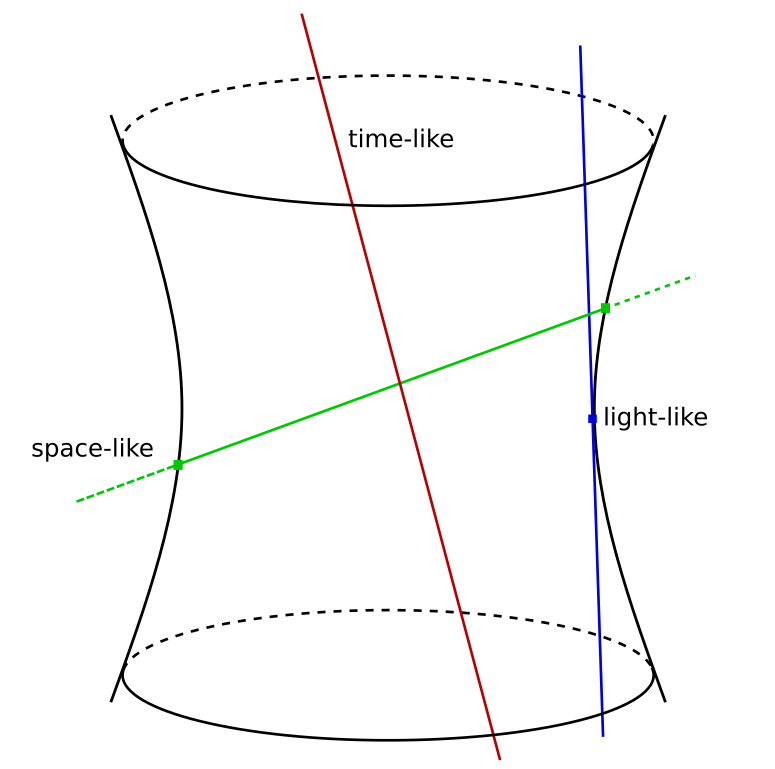
\includegraphics[width=0.7\textwidth]{baleani.png}
    \caption{Geodesics in $\A^{2,1}$}
    \label{projchart}
\end{figure}

In particular, the light cone through a point $\left[ x \right] \in \A^{n,1}$ coincides with the cone of lines through $\left[ x \right]$ tangent to $\partial \A^{n,1}$.\\
In an affine chart, timelike geodesics correspond to affine lines which are entirely contained in the Anti de Sitter space, and which are not asymptotic to its boundary; lightlike geodesics are tangent to the one-sheeted hyperboloid, or are asymptotic to it.\\

\noindent \textit{Totally geodesic subspaces}. Let us briefly discuss more in general totally geodesics subspaces. By an argument analogous to the case of geodesics, totally geodesic subspaces of $\A^{n,1}$ of dimension $k$ are obtained as the intersection of $\A^{n,1}$ with the projectivisation $P(W)$ of a linear subspace $W$ of $\R^{n,2}$ of dimension $k+1$. The negative index of $W$ can be either $2$ or $1$, for otherwise the intersection $\A^{n,1}\cap P(W)$ would be empty.
We have several cases
\begin{itemize}
    \item If $W$ has signature $(k-1,2)$, then $P(W)\cap\A^{n,1}$  is isometric to $\A^{k-1,1}$.
    \item If $W$ has signature $(k-2,1)$, then it is a copy of Minkowski space $\R^{k-2,1}$, hence $P(W)\cap\A^{n,1}$ is a copy of the Klein model of hyperbolic space.
    \item If $W$ is degenerate, then $P(W)\cap\A^{n,1}$ is a lightlike subspace foliated by lightlike geodesics tangent to the same point of $\partial\A^{n,1}$. 
\end{itemize}

\noindent \textit{In the universal cover}. In the universal cover $\AS^{n,1}$ geodesics are the lifts of the geodesics of $\H^{n,1}$ or $\A^{n,1}$. Every lightlike or spacelike geodesic in $\H^{n,1}$ and $\A^{n,1}$ is topologically a line, therefore it has a countable number of lifts to $\AS^{n,1}$, On the other hand timelike geodesics $\H^{n,1}$ and $\A^{n,1}$ are topologically circles and are in bijection with timelike geodesics of $\AS^{n,1}$.\\
Using the Poincaré model we can give an explicit description of lightlike geodesics. In fact, in Lorentzian geometry not only the nature of a vector is conformally invariant but also unparametrized lightlike geodesics are a conformal property (\cite{Gallot}, Proposition 2.131): 
 \begin{theorem}\label{ConformalMetric} If two Lorentzian metrics $g,g^{\prime} $ on a manifold $M$ are conformal, then they have the same unparametrized lightlike geodesics.
 \end{theorem}

Because of Theorem \ref{ConformalMetric} we can replace the Poincaré metric by the conformally equivalent metric, and often more easy to manage in calculation, given by:
 \begin{equation}\label{hemispherical}
     \frac{4}{(1+r^2)^2}(dx_1^2+\dots+dx_n^2)-dt^2
 \end{equation} 
 Now we observe that the first term in Equation \ref{hemispherical} is exactly the form of the spherical metric on a hemisphere, pulled-back to the unit disk by the stereographic projection. We call such a metric hemispherical and we denote it by $g_{\mathbb{S}^n}$. Notice that the boundary of $\D^n$ is an equator for the hemispherical metric, and in fact it is the only equator completely contained in $(\D^n\cup\partial\D^n,g_{\mathbb{S}^n})$, a justification to the fact that we refer to it as \textit{the} equator.\\
 As a consequence, unparametrized lightlike geodesics of $\AS^{n,1}$, going through a point $(p_0,t_0)$ are characterized by the condition that they are mapped to spherical geodesic under the vertical projection $(p,t)\to p$ and moreover
 \[
     t-t_0=d_{\mathbb{S}^n}(p,p_0)
 \] on the geodesic. In particular, these lightlike geodesics meet the boundary of $\AS^{n,1}$ at the point that satisfies the above conditions such that $p$ is on the equator of the hemisphere: as an example, if $p_0$ is the center of the hemisphere, then the points at infinity of the lightcone over $(p_0,t_0)$ are the horizontal slices $t=t_{0}+\pi/2.$ This sphere is also the boundary of a hyperplane dual to $(p_0,t_0)$, in a sense that we will explain in the following section. \\
 By an analogous reasoning we can give an explicit description of a lightlike hyperplane in the Poincaré model: the lightlike plane having $(p_0,t_0)$ as a past endpoint, (where now $p_0$ is on the equator) is precisely $\{(p,t)\;|\;t-t_0=d_{\mathbb{S}^n}(p,p_0)\}$ and its future endpoint is $(-p_0,t+\pi.)$ 

\section{Polarity in Anti-de Sitter space} \label{sec:reg}
The quadratic form $q_{n,2}$ induces a polarity on the projective space $\mathbb{R} \text{P}^{n,1}$, namely the correspondance which associates to the projective subspace $P(W)$ the subspace $P(W^ \perp)$. In particular this induces a duality between spacelike totally geodesic subspaces of $\A^{n,1}$: the dual of a spacelike $k$-dimensional subspace is a $n-k+1$-dimensional subspace.
We indicate with $P_{[x]}=P(x^\perp)$ the hyperplane dual to a point $[x]\in \A^{n,1}$.
Projectively $P_{[x]}$ is characterised as the hyperplane spanned by the intersection of $\partial\A^{n-1,1}$ with the lightcone from $[x]$.
More geometrically, it can be checked that $P_{[x]}$ is the set of antipodal points to $[x]$ along timelike geodesics through $[x]$. Also, every timelike geodesic
through $[x]$ meets $P_{[x]}$ orthogonally at time $\pi/2$. Conversely, given a totally geodesic spacelike hyperplane $H$, all the timelike geodesics that meet $H$ orthogonally  intersect in a single point, which is the dual point of $H$.\\
To some extent, this duality between points and planes lifts to the coverings of $\A^{n,1}$.\\

\noindent\textit{In the quadric model}. In $\H^{n,1}$ there are two dual planes associated to any point $x$: the sets 
\[
P_{x}^\pm=\{\exp_{x}(\pm(\pi/2)v)\,|\,q_{n,2}(v)=-1,\,v\text{ future-directed}\}~.
\]
Clearly $P_{x}^+$ and $P_{x}^{-} $ are antipodal and  $P_{-x}^\pm=P_{x}^\mp$. The planes $P_x^{\pm}$ disconnect $\H^{n,1}$ in two regions $U_x$ and
$U_{-x}$, where $U_{x}$ is the region containing $x$. They can be characterised by 
\[
U_{x}=\{y\in\H^{n,1}\,|\,\langle x, y\rangle_{n,1}<0\}.
\]

Spacelike and lightlike geodesics through $x$ do not exit $U_{x}$, 
while all the timelike geodesics through $x$ meet orthogonally $P^{\pm}_x$ and all pass through the point $-x$.
More precisely, a point $y\neq x$ is connected to $x$:
\begin{itemize}
\item by a spacelike geodesic if and only if $\langle x,y\rangle_{n,1}<-1$,
\item by a lightike geodesic if and only if $\langle x,y\rangle_{(n,1)}=-1$,
\item by a timelike geodesic if and only if 
$|\langle x,y\rangle_{(n,1)}|<1$.
\end{itemize}
An immediate consequence is that if $y$ is connected to $x$ by a spacelike geodesic, there is no geodesic joining $y$ to $-x$.
Hence the exponential map of $\H^{n,1}$ is not surjective. But as any point $y\in\H^{n,1}$ can be connected through a geodesic either to $x$ or to $-x$,
the exponential over $\A^{n,1}$ is surjective.\\

\noindent\textit{In the universal cover}.
Recall that the group of deck transformations for the covering $\AS^{n,1} \to \H^{n,1}$ is $\Z$, where a generator acts by translations of $2\pi$ in the $\R$ factor. Hence the  preimage of a spacelike plane $P\subset\A^{n,1}$ is the disjoint union of spacelike planes $(P^k)_{k\in\Z}$, enumerated so that the generator $\eta$ of $\Z$ acts by sending $P^k$ to $P^{k+1}$.
Moreover each connected component of $\A^{n,1}\setminus\bigcup_{k\in\Z}P^k$ is a fundamental  domain for the action of deck transformations of the covering $\AS^{n,1}\to\A^{n,1}$.\\
Take now $x\in \AS^{n,1}$ and apply the construction above with $P = P_{\pi'(x)}$ the plane dual to $\pi'(x)$ in $\A^{n,1}$. We refer to the connected component of $\AS^{n,1} \setminus \bigcup_{k\in\Z}P_{\pi'(x)}^k$ containing $x$ as the \textit{Dirichlet domain} $R_x$ of $x$. By a small abuse of notation, we also denote the planes that bound $R_x$ by $P^+_x$ and $P^-_x$.
